\documentclass[12pt, 
hyperref={colorlinks=true, linkcolor=blue, urlcolor=cyan}]{beamer}
\usetheme{default} 

\setbeamertemplate{navigation symbols}{} %gets rid of navigation symbols
\setbeamertemplate{footline}{} %gets rid of bottom navigation bars
\setbeamertemplate{footline}[page number]{} %use this for page numbers

\setbeamertemplate{footline}{%
  \raisebox{5pt}{\makebox[\paperwidth]{\hfill\makebox[10pt]{\scriptsize\insertframenumber~~}}}}

\setbeamertemplate{itemize items}[circle] %round bullet points
\setlength\parskip{10pt} % white space between paragraphs

\usepackage{wrapfig}
\usepackage{subfig}
\usepackage{setspace}
\usepackage{enumerate}
\usepackage{graphicx}
\usepackage{amsmath}
\usepackage{amsfonts}
\usepackage{amssymb}
\usepackage{amsthm}
\usepackage[UKenglish]{isodate}
\usepackage{tikz}
\usepackage{natbib}
\def\checkmark{\tikz\fill[scale=0.4](0,.35) -- (.25,0) -- (1,.7) -- (.25,.15) -- cycle;} 

% bracketing shortcuts
\newcommand{\paren}[1]{\left(#1\right)}
\newcommand{\sqbracket}[1]{\left[#1\right]}
\newcommand{\cbracket}[1]{\left\{#1\right\}}
\newcommand{\abs}[1]{\left\lvert#1\right\rvert}
\newcommand{\norm}[1]{\left\lVert#1\right\rVert}
% set up the argmin operator, argmax
\DeclareMathOperator*{\argmin}{arg\,min}
\DeclareMathOperator*{\argmax}{arg\,max}

\newcommand{\myframe}[1]{\begin{frame} \frametitle{#1}}
% the preamble
\title{Unix systems/shell scripting/cluster computing}
\author{Brian Williamson}
\institute{BIOST 561: Computational Skills For Biostatistics I}
\date{16 November 2017}

% Start the document
\begin{document}
% The title page
\begin{frame}
\titlepage
\end{frame}

\section{Motivation}
\myframe{Unix systems/shell scripting}
\begin{columns}[c]
\begin{column}{.66\textwidth}
\vspace{1cm}

\emph{Since there seems to be no hope of C becoming
an expression language (in which case it would be
potentially more suitable for the shell) there is
equally no hope that the shell and C will be the
same language.}

\vspace{2cm}
\href{https://en.wikipedia.org/wiki/Stephen_R._Bourne}{Stephen R. Bourne} (1977, from a talk in 2015)

British computer scientist, author of the Bourne shell (\texttt{sh})  
\end{column}
\begin{column}{.33\textwidth}
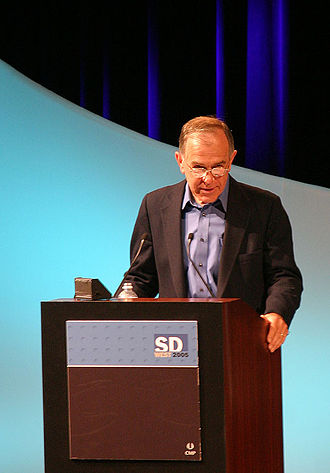
\includegraphics[width=1\textwidth]{bourne.jpg}
\end{column}
\end{columns}
\end{frame}

% Motivation: typical R use, clusters are Linux
\myframe{Motivation}
Why not keep running R using a GUI and (R) scripts?
\begin{itemize}
\item \textcolor{red}{Requires keeping R/RStudio open while the script is running}
\item[]
\item Can take up \textcolor{red}{significant resources} on a personal machine
\item[]
\item May need to open \textcolor{red}{multiple R/RStudio windows to run multiple jobs} (there are some ways around this)
\end{itemize}

Many courses (e.g., 570s) and research will require a more sophisticated approach.
\end{frame}

\myframe{The solution!}
The department has \emph{cluster computers} for just this purpose!

Cluster computers:
\begin{itemize}
\item Allow you to \textcolor{blue}{submit multiple jobs at once}
\item[]
\item Depending on the system, \textcolor{blue}{can schedule jobs for you}
\item[]
\item Are \textcolor{blue}{optimized for high-throughput performance}
\end{itemize}
\end{frame}

\section{Unix systems}
% Unix systems: little bit of history, how to navigate. also linux
\myframe{Unix systems}
Three common types of laptop/desktop operating systems: Windows, Mac, Linux.

Mac and Linux are both Unix-like!

What that means for us: Unix-like operating systems are equipped with ``shells'' that provide a command line user interface.

\centering

\includegraphics[width=0.5\textwidth]{unix.png}
\hspace{2cm}

\includegraphics[width=0.25\textwidth]{linux.png}
\end{frame}

\myframe{Navigating Unix/Linux}
Some useful commands (\href{http://stackoverflow.com/}{StackOverflow} has more!):

\begin{tabular}{|l|l|}
Command & Purpose \\
\hline
mkdir & create new directory \\
rmdir & remove a directory \\
cd & change directory \\
pwd & print current working directory (cwd) \\
ls & list all files and folders in cwd \\
mv & rename or move a file \\
cp & copy a file \\
rm & remove a file \\
ps & list running processes \\
top & print running update\\
cat & display a text file \\
more & display any file
\end{tabular}
\end{frame}

\myframe{Navigating Unix/Linux}
Some useful shortcuts/more commands (\href{http://stackoverflow.com/}{StackOverflow} has more!):

\begin{tabular}{|l|l|}
Shortcut & Purpose \\
\hline
* & select all items in the cwd \\
. & look in the cwd \\
.. & look in the parent directory \\
chmod & change permissions for a file \\
./\texttt{program.sh} & run the executable file \texttt{program.sh}
\end{tabular}

Your best friend is Google if you run into problems!

\end{frame}

\section{Running GUI-less}
% ONLY THE HIGHLIGHTS
\myframe{Running GUI-less: the highlights}
There are many nuances to running GUI-less (see the other set of slides), but here are a few of the highlights:
\begin{itemize}
\item \textcolor{blue}{Set a seed!} This ensures that your results are reproducible (by you and others)
\item Think hard about what output you want to save, and \textcolor{blue}{save it manually} either in your R script or in a shell script
\item Tell the computer where to look for the executable file to run your code (using a \texttt{\#!})
\item R scripts (and the \texttt{Rscript} executable) can take parameters passed from the command line
\end{itemize}
\end{frame}

\begin{frame}[fragile]
\frametitle{Example: Robust SEs}
Consider a sample of $n$ observations generated according to
\begin{align*}
X_i &\stackrel{i.i.d.}{\sim} N(0, 1), \\
u_i &\stackrel{i.i.d.}{\sim} N(0, 1), \text{ independent of the } X_i, \\
Y_i \mid X_i, u_i &= \beta_0 + \beta_1 X_i + \epsilon_i, \text{ where} \\
\epsilon_i &= \abs{X_i}u_i.
\end{align*}

Suppose we wish to estimate $\beta_1$ using linear regression. We clearly have some heteroskedasticity, so we can compare coverage of 95\% CIs using model-based and robust standard errors for $\hat{\beta_1}$.
\end{frame}

\begin{frame}[fragile]
\frametitle{Robust SEs: the \texttt{doOne()} function}
{\scriptsize
\begin{verbatim}
doOne <- function(n, beta) {
  ## create the data
  x <- rnorm(n, 0, 1)
  u <- rnorm(n, 0, 1)
  eps <- abs(x)*u
  beta0 <- 1
  y <- beta0 + beta*x + eps
  
  ## fit the linear regression model
  mod <- lm(y ~ x)
  
  ## extract model coefficients and SEs
  est <- coefficients(mod)[2]
  se <- vector("numeric", 2)
  se[1] <- sqrt(diag(vcov(mod)))[2]
  se[2] <- sqrt(diag(vcovHC(mod, "HC0")))[2]
  
  ## Create CIs
  ci <- est + se %o% qnorm(c(0.025, 0.975))
  cover <- beta > ci[, 1] & beta < ci[, 2]
  names(cover) <- c("Model", "Sandwich")
  
  ## return
  return(c(est, cover))
}
\end{verbatim}
}
\end{frame}

\begin{frame}[fragile]
\frametitle{Script \texttt{se\_ex1.R}}
{\fontsize{9pt}{7.2}\selectfont
\begin{verbatim}
#!/usr/local/bin/Rscript
args <- commandArgs(TRUE)
## Parse the arguments
if(length(args) == 0) {
  print("No arguments supplied.")
} else {
  for (i in 1:length(args)) {
    eval(parse(text = args[i]))
  }
}
if(!exists("truebeta")) {
  truebeta <- 2
  cat("\n Note: Assmuming truebeta = 2 \n")
}
if(!exists("n")) {
  n <- 500
  cat("\n Note: Setting n = 500 \n")
}
if(!exists("seed")) {
  seed <- 547
  cat("\n Note: Setting seed = 547 \n")
}
if(!exists("B")) {
  B <- 1000
  cat("\n Note: setting B = 1000 \n")
}
\end{verbatim}
}
\end{frame}

\begin{frame}[fragile]
\frametitle{Script \texttt{se\_ex1.R} (continued)}
{\scriptsize
\begin{verbatim}
doOne <- function(n, beta) {
 <See previous slide>
}
library(sandwich)
set.seed(seed)
system.time(output <- replicate(B, doOne(n = n, beta = truebeta)))
apply(output, 1, mean)
\end{verbatim}
}
\end{frame}

\begin{frame}[fragile]
\frametitle{Running jobs: Rscript}
On Box (or Cox, more on this later) we can run jobs using Rscript. For the SE example:
{\scriptsize
\begin{verbatim}
[brianw26@cox ~/biost_561]$ Rscript se_ex1.R > ex1_output.txt B=10000 
seed=547 n=500 truebeta=2
\end{verbatim}}
 ... which creates an object \texttt{ex1\_output.txt} containing all of the output we saved (only the average values and the system time).

Nothing else is saved! Takes 43 seconds (would take longer, perhaps, on a personal computer or on Box). \textcolor{red}{Do you expect things would take longer if we also were getting bootstrap CIs? How much longer?}
\end{frame}

\begin{frame}[fragile]
\frametitle{Running jobs: multiple jobs at once}
If we need to set off a collection of R processes, we can use \texttt{\&} at the end of a line to allow entry of another line, e.g., 
{\scriptsize
\begin{verbatim}
[brianw26@cox ~/biost_561]$ Rscript se_ex1.R > ex1_output_200.txt B=10000 
seed=547 n=200 truebeta=2 &
[1] 755
[brianw26@cox ~/biost_561]$ Rscript se_ex1.R > ex1_output_500.txt B=10000 
seed=547 n=500 truebeta=2 &
[2] 786
\end{verbatim}
}
\end{frame}

\subsection{Running multiple jobs}
\begin{frame}[fragile]
\frametitle{Running jobs: multiple jobs at once}
Or, we can write a shell script! This is especially useful if we need to set off multiple jobs at once, or we have different settings that our simulation needs to run with. 
\begin{enumerate}
\item Make a script file of command-line commands (not R), e.g., 
\begin{verbatim}
#!/bin/sh
Rscript myscript.R n=100 seed=147 &
Rscript myscript.R n=300 seed=347 &
Rscript myscript.R n=500 seed=547
\end{verbatim}
and save this off as \texttt{myMasterScript.sh}
\item[]
\item \texttt{chmod u+x myMasterScript.sh} grants Yo\textbf{u}, the file owner, permission to e\textbf{x}ecute the file
\item[]
\item \texttt{./myMasterScript.sh} runs the script
\end{enumerate}
\end{frame}

\begin{frame}[fragile]
\frametitle{Example: robust SE shell script}
For the robust SE example, this would be 
{\scriptsize
\begin{verbatim}
[brianw26@cox ~/biost_561]$ more se_ex1.sh
#!/bin/sh

Rscript se_ex1.R > ex1_output_n_100.txt B=10000 
seed=101 n=101 truebeta=2 &
Rscript se_ex1.R > ex1_output_n_300.txt B=10000 
seed=301 n=101 truebeta=2 &
Rscript se_ex1.R > ex1_output_n_500.txt B=10000 
seed=501 n=101 truebeta=2 &

[brianw26@cox ~/biost_561]$ chmod u+x se_ex1.sh
[brianw26@cox ~/biost_561]$ ./se_ex1.sh
\end{verbatim}
}
\end{frame}

% bootstrap vs permutation test
\begin{frame}[fragile]
\frametitle{Example: robust vs model-based SEs}
After 43 seconds, we get the following output (what could we have saved to make things slightly more interesting?)

\begin{verbatim}
[brianw26@cox ~/biost_561]$ cat ex1_output.txt
     user  system   elapsed
   43.167  0.008    43.172
       x    Model   Sandwich
1.999183 0.738700   0.948900
\end{verbatim}
\end{frame}

\begin{frame}[fragile]
\frametitle{Example: robust vs model-based SEs \small (interesting?)}
Here's some code$^*$ from the end of an R script that saves off the coefficient estimates and whether or not the CI covers the truth: 
{\scriptsize
\begin{verbatim}
library(sandwich)
set.seed(seed)
system.time(output <- replicate(B, doOne(n = n, beta = truebeta)))
# apply(output, 1, mean)
saveRDS(file=paste("ex3_output_n_", n, "_beta_", truebeta, "_b_", B, 
                "_seed_", seed, ".rds", sep = ""))
\end{verbatim}
}

\textcolor{blue}{What would we additionally need to save to re-construct the CIs?} (besides saving the CIs themselves)

\small
${}^*$ the rest is the same as \texttt{se\_ex1.R}
\end{frame}

\begin{frame}
\frametitle{Example: robust vs model-based SEs \small (interesting?)}
% PICTURES OF THE SAMPLING DISTRIBUTIONS, PERCENT COVER
\centering
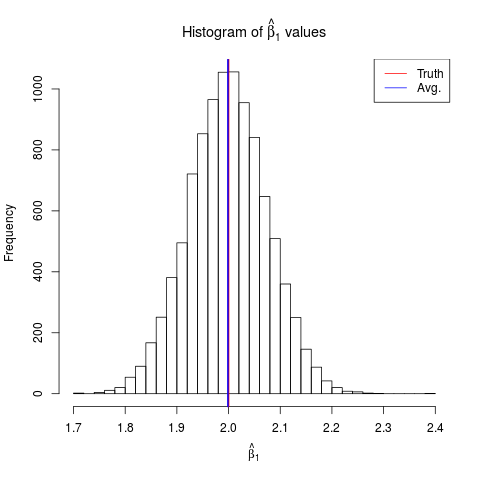
\includegraphics[width = 0.6\textwidth]{se_ex3_beta_ests.png}
\small

\begin{tabular}[t]{l|r|r}
\hline
  & Model-based & Sandwich\\
\hline
Coverage & 0.748 & 0.9494\\
\hline
\end{tabular}
\end{frame}

\section{Cluster computing and shell scripting}
% CLUSTERS
\myframe{Cluster computing/shell scripting}
\begin{columns}[c]
\begin{column}{.66\textwidth}
\vspace{1cm}

\emph{When I was younger, I thought of myself as a pretty good programmer...}

\vspace{2cm}
\href{http://www.software-engin.com/}{Ian Sommerville} (2015)

Scottish computer scientist
\end{column}
\begin{column}{.33\textwidth}
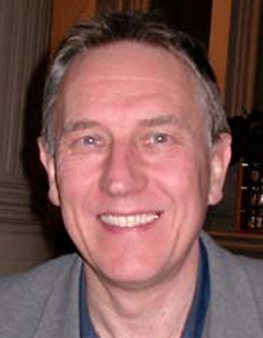
\includegraphics[width=1\textwidth]{sommerville.jpg}
\end{column}
\end{columns}
\end{frame}

\myframe{Cluster computing}
All of us can constantly improve our programming.

In addition to learning new languages (e.g., shell), we can also learn new ways to speed up/optimize code.

The clusters allow us to do the latter.
\end{frame}

\myframe{Running GUI-less: on to the clusters}
Sometimes (all the time) we do not want to leave a R session open on our laptop while a simulation runs.

There are two main shared department resources for computing (in my experience): Cox (not a cluster) and Bayes (a cluster).

\begin{itemize}
\item Cox: 12 core computer 
\item[]
\item Bayes: 
\begin{itemize}
\item Compute cluster with 4 compute nodes, each with 12 cores (additional PI-specific nodes)
\item Designed for high-throughput computing
\item Managed by Sun Grid Engine (SGE)
\end{itemize}
\end{itemize}
\centering
%\includegraphics[width = 0.15\textwidth]{david_cox.jpg}\hspace{1cm} \includegraphics[width = 0.2\textwidth]{bayesandmendel.jpg}
\end{frame}

% How to use the cluster: logging on, submitting jobs, checking jobs, etc.
\myframe{Logging on to a cluster: Windows (including Box)}
\begin{enumerate}
\item Open Tera Term [or your favorite secure shell (SSH) client]
\item Enter the address of your favorite cluster, e.g., \texttt{bayes.biostat.washington.edu}
\item Make sure that the ``New connection'' window is filled out as in the figure, except for ``Host'' (on Box things are different)
\item Click \texttt{OK}, enter your UW BIOST username and password when prompted (the user and pass you use to log in to Box) 
\end{enumerate}
\centering
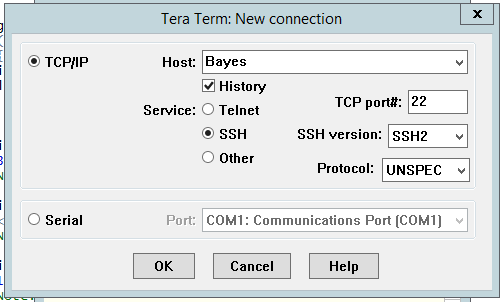
\includegraphics[width = .45\textwidth]{tera_term_example.png}
\end{frame}

\myframe{Logging on to a cluster: Mac/Linux}
\begin{enumerate}
\item Open a Terminal window
\item[]
\item Type \texttt{ssh mynetid@cluster.washington.edu}
\begin{itemize}
\item replace \texttt{mynetid} with Your UW NetID, and 
\item replace \texttt{cluster} with Your cluster, e.g., \texttt{bayes}
\end{itemize} 
\item[]
\item Enter password (same password as Box login) when prompted --- the field will remain blank but your password will be received
\end{enumerate}
\end{frame}

\myframe{Using the clusters}
Once logged in, navigation is always the same, since the clusters are all Unix based!

All files from your \texttt{P:/} drive are on every cluster

Now we can use all of those commands from slides 6--7. However, how we run ``jobs'' depends on the cluster:
\begin{itemize}
\item Cox: one job at a time (basically)
\item[]
\item Bayes: many jobs at once, scheduled by SGE
\end{itemize}
\end{frame}

\begin{frame}[fragile]
\frametitle{Using the clusters: Windows file compatability}
Sometimes we can run into errors when running files on Unix machines. A place where I often go wrong is by \textcolor{red}{saving files in Windows and then trying to run the file on Unix}.

A common type of error comes from \emph{control characters}, commonly seen as end of line characters in Windows. For the permutation test example:
{\scriptsize
\begin{verbatim}
[brianw26@cox ~/biost_561]$ ./perm_test_2.sh
./perm_test_2.sh: Command not found.
[brianw26@cox ~/biost_561]$ cat -vt ./perm_test_2.sh
#!/bin/sh^M
Rscript permutation_test_example_guiless.R myn=100 myseed=101 myB=10000 &^M
Rscript permutation_test_example_guiless.R myn=300 myseed=301 myB=10000 &^M
Rscript permutation_test_example_guiless.R myn=500 myseed=501 myB=10000^M
\end{verbatim}
} 
To run our script successfully, we need to remove these characters either \textcolor{red}{by hand using \texttt{vim} or \texttt{emacs} to edit the file}, or by running \textcolor{blue}{\texttt{dos2unix myfile.sh}}.
\end{frame}

\myframe{Using the clusters: being nice}
The department clusters are shared resources, here for our benefit. There are a few ways to be nice about how you use the clusters:
\begin{enumerate}
\item Bayes is a compute cluster --- one head node (schedules jobs) hooked up to compute nodes (run the jobs). Bayes is optimized to run jobs on the compute nodes, not the head node. \textcolor{red}{Do not run memory-intensive or long jobs on the head node!}
\item[]
\item Submitting jobs on Bayes automatically ``nices'' for you --- SGE lowers your priority as your number of currently running jobs increases, and increases priority again as jobs finish running
\item[]
\item Running long/memory-intensive jobs on Cox slows down the computer for all users 
\end{enumerate}
\end{frame}

\subsection{Running a single job}
\subsection{Single job: Bayes}
\begin{frame}[fragile]
\frametitle{Running a single job on Bayes}
Write a shell script that calls your function(s). For example:
\vspace{-.5cm}{\fontsize{9pt}{7.2}\selectfont \begin{verbatim}
[brianw26@bayes0 ~/biost_561]$ more call_ex1.sh
#!/bin/sh

Rscript se_ex1.R > ex1_output.txt B=10000 seed=547 n=500 truebeta=2
\end{verbatim}
}
\begin{itemize}
\item The first line tells Bayes to run using the Bourne shell (sh). You can change this to another shell if you want
\item The script calls Rscript to run the file \texttt{se\_ex1.R} and pipes any output to \texttt{ex1.output.txt}
\item The values \texttt{B=10000} etc. are command line arguments
\end{itemize}

To submit the job:
\vspace{-.5cm}{\fontsize{9pt}{7.2}\selectfont \begin{verbatim}
[brianw26@bayes0 ~/biost_561]$ qsub -cwd call_ex1.sh
Your job 3875039 ("call_ex1.sh") has been submitted
\end{verbatim} }
\end{frame}

\myframe{Submitting jobs on Bayes}
There are many options for \texttt{qsub}. A few examples:
\begin{itemize}
\item \texttt{-cwd} executes the script in the current working directory
\item \texttt{-e} and \texttt{-o} can be used to send error and output files (from \texttt{qsub}, not R) to a folder, e.g., \texttt{iotrash/}
\item \texttt{-N} names a job
\item \texttt{-t <tasklist>} submits a job array
\end{itemize}

See the \href{http://gridscheduler.sourceforge.net/htmlman/htmlman1/qsub.html}{manual} for more detailed information. 
\end{frame}

\begin{frame}[fragile]
\frametitle{Submitting jobs on Bayes: options}
You can also set defaults in Your home directory (e.g., \texttt{P:/}) in a file called \texttt{.sge\_request}. These also come from the \href{http://gridscheduler.sourceforge.net/htmlman/htmlman1/qsub.html}{manual}. Mine is
\begin{verbatim}
-j y
-cwd
-S /bin/bash
-q normal.q
-M brianw26@uw.edu
-m e
\end{verbatim}

\begin{itemize}
\item \texttt{-j y} says that I can submit a binary or script file
\item \texttt{-S} tells SGE the default program to run my script
\item \texttt{-q} tells SGE which queue to run my script on
\item \texttt{-M} tells SGE who to email (me)
\item \texttt{-m} tells SGE when to email (\texttt{e} is end of job)
\end{itemize}
\end{frame}

\myframe{Checking/altering jobs on Bayes}
Once you have submitted a job, there are many options for checking/altering it:
\begin{itemize}
\item \texttt{qstat} checks queue status
\begin{itemize}
\item \texttt{-f} shows full status of jobs
\item \texttt{-u <user>} shows status of jobs for user \texttt{user}
\item \texttt{-j <job\_id>} gives details about a single job
\end{itemize}
\item \texttt{qhold <job\_id>[.tasklist]} puts a hold on job \texttt{job\_id} (and optionally array elements in \texttt{tasklist} --- more on this later)
\item \texttt{qrls <job\_id>} removes a hold on a job
\item \texttt{qdel <job\_id>} deletes a job
\end{itemize}
\end{frame}

\subsection{Multiple jobs: Bayes}
\myframe{Submitting multiple jobs to Bayes}
An alternative to submitting multiple jobs by hand, or parallelizing code directly, is to submit a batch of individual jobs to Bayes. Advantages:
\begin{itemize}
\item This is what Bayes is set up for
\item It is a simple way to run a set of simulations using varying parameters (I do this all the time)
\end{itemize}

I recommend including seed number and other parameter values in the filename used to save output. This makes it easy to loop over saved output/objects to combine output later.
\end{frame}

\begin{frame}[fragile]
\frametitle{Submitting multiple jobs to Bayes: loops}

Create a submission script that loops over arguments: 
{\scriptsize
\begin{verbatim}
[brianw26@bayes0 ~/biost_561]$ more submit_ex1_batch.sh
#!/bin/sh

B=5000
seed=47

for n in 100 300 500
do
for truebeta in {1..5}
do
    qsub -cwd -e iotrash/ -o iotrash/ -q normal.q@b01.local ./call_ex1_once.sh
$B $seed $n $truebeta
done
done
\end{verbatim}
}

NB: You'll need to create a folder in your \texttt{cwd} called \texttt{iotrash}, and make \texttt{call\_ex1\_once.sh} executable for this to work.
\end{frame}

\begin{frame}[fragile]
\frametitle{Submitting multiple jobs to Bayes: loops}
Write your script to accept command line parameters:
{\fontsize{9pt}{7.2}\selectfont
\begin{verbatim}
[brianw26@bayes0 ~/biost_561]$ more call_ex1_once.sh
#!/bin/sh

Rscript se_ex1.R > ex1_output_b$1_s$2_n$3_beta$4.txt B=$1 seed=$2 n=$3 
truebeta=$4
\end{verbatim}
}
The values of \texttt{\$1}, \texttt{\$2}, $\dots$, \texttt{\$n} are the 1st, 2nd, $\dots$, \texttt{n}th command line arguments.

In this example, four arguments are passed to the \texttt{se\_ex1.R} script and they are included in the file name.
\end{frame}

\begin{frame}[fragile]
\frametitle{Submitting multiple jobs to Bayes: job arrays}
An alternative to using a shell script loop is to submit your job as a job array. Each job array task has a unique ID, which you can read in to set up a simulation.

To do this successfully, your R script has to contain a matrix with all combinations of simulation parameters that you want to run over. Here's a chunk from \texttt{se\_ex2.R}:
{\scriptsize
\begin{verbatim}
#!/usr/local/bin/Rscript

doOne <- function(n, beta) {
<Code omitted -- see previous slide>
}

## get the array task id
job.id <- as.numeric(Sys.getenv("SGE_TASK_ID"))

## set up simulation parameters
ns <- c(100, 300, 500)
B <- 5000
truebetas <- seq(1, 5, 1)
\end{verbatim}
}
\end{frame}

\begin{frame}[fragile]
\frametitle{More from \texttt{se\_ex2.R}}
{\scriptsize
\begin{verbatim}
param.grid <- expand.grid(ns, truebetas)
param.grid$B <- B
param.grid$seed <- param.grid[, 1] + param.grid[, 2]
names(param.grid) <- c("n", "truebeta", "B", "seed")

current <- param.grid[job.id, ]
library(sandwich)
set.seed(current$seed)
system.time(output <- replicate(B, doOne(n = current$n, 
                                         beta = current$truebeta)))
save(output, file = paste("ex2_output_b_", current$B, "_s_", 
                          current$seed, "_n_", current$n, 
                          "_beta_", current$truebeta, sep = ""))
\end{verbatim}
}
\end{frame}

\begin{frame}[fragile]
\frametitle{Submitting multiple jobs to Bayes: job arrays}
Once your R script can handle submission as a job array, set up a script to call it once and then a script to submit it as a job array, e.g.,
{\scriptsize
\begin{verbatim}
[brianw26@bayes0 ~/biost_561]$ more call_ex2_once.sh
#!/bin/sh

Rscript se_ex2.R
\end{verbatim}
\begin{verbatim}
[brianw26@bayes0 ~/biost_561]$ more submit_ex2_batch.sh
#!/bin/sh

qsub -t 1-15 -cwd -e iotrash/ -o iotrash/ -q normal.q -l "h=b01|b02|b03|b04" 
-shell no -b yes ./call_ex2_once.sh
\end{verbatim}
}
\end{frame}

\myframe{Submitting multiple jobs to Bayes: being nice}
Remember that Bayes is a shared resource. If you find the cluster empty, and fill up all of the nodes with long jobs, remember to \textbf{monitor} these jobs and the queue and be prepared to suspend some of those jobs as other users' jobs enter the queue. A good rule of thumb is to only have \textcolor{red}{20 jobs running at a single time}.

Ways to help share the cluster:
\begin{itemize}
\item Submit batch jobs in job arrays --- this makes the queue easier for everyone to read
\item Use manual holds or link automatic holds on jobs, using the \texttt{-tc} argument in \texttt{qsub}
\item Reduce priority of jobs if necessary
\item Estimate how long each job will take, and take this into consideration when submitting large batches
\end{itemize}
\end{frame}

\end{document}
